

Đơn vị số học và logic (ALU) là thành phần thực thi các phép toán cốt lõi của CPU. Mặc dù hệ thống sử dụng định dạng mã hóa lệnh 8-bit (3-bit Opcode và 5-bit Operand), nhưng khối ALU được thiết kế để xử lý dữ liệu với độ rộng thực tế là \textbf{32-bit}. Điều này cho phép máy tính thực hiện các phép tính trên dải giá trị lớn, đáp ứng tiêu chuẩn của các kiến trúc máy tính hiện đại.

\begin{figure}[H]
    \centering
    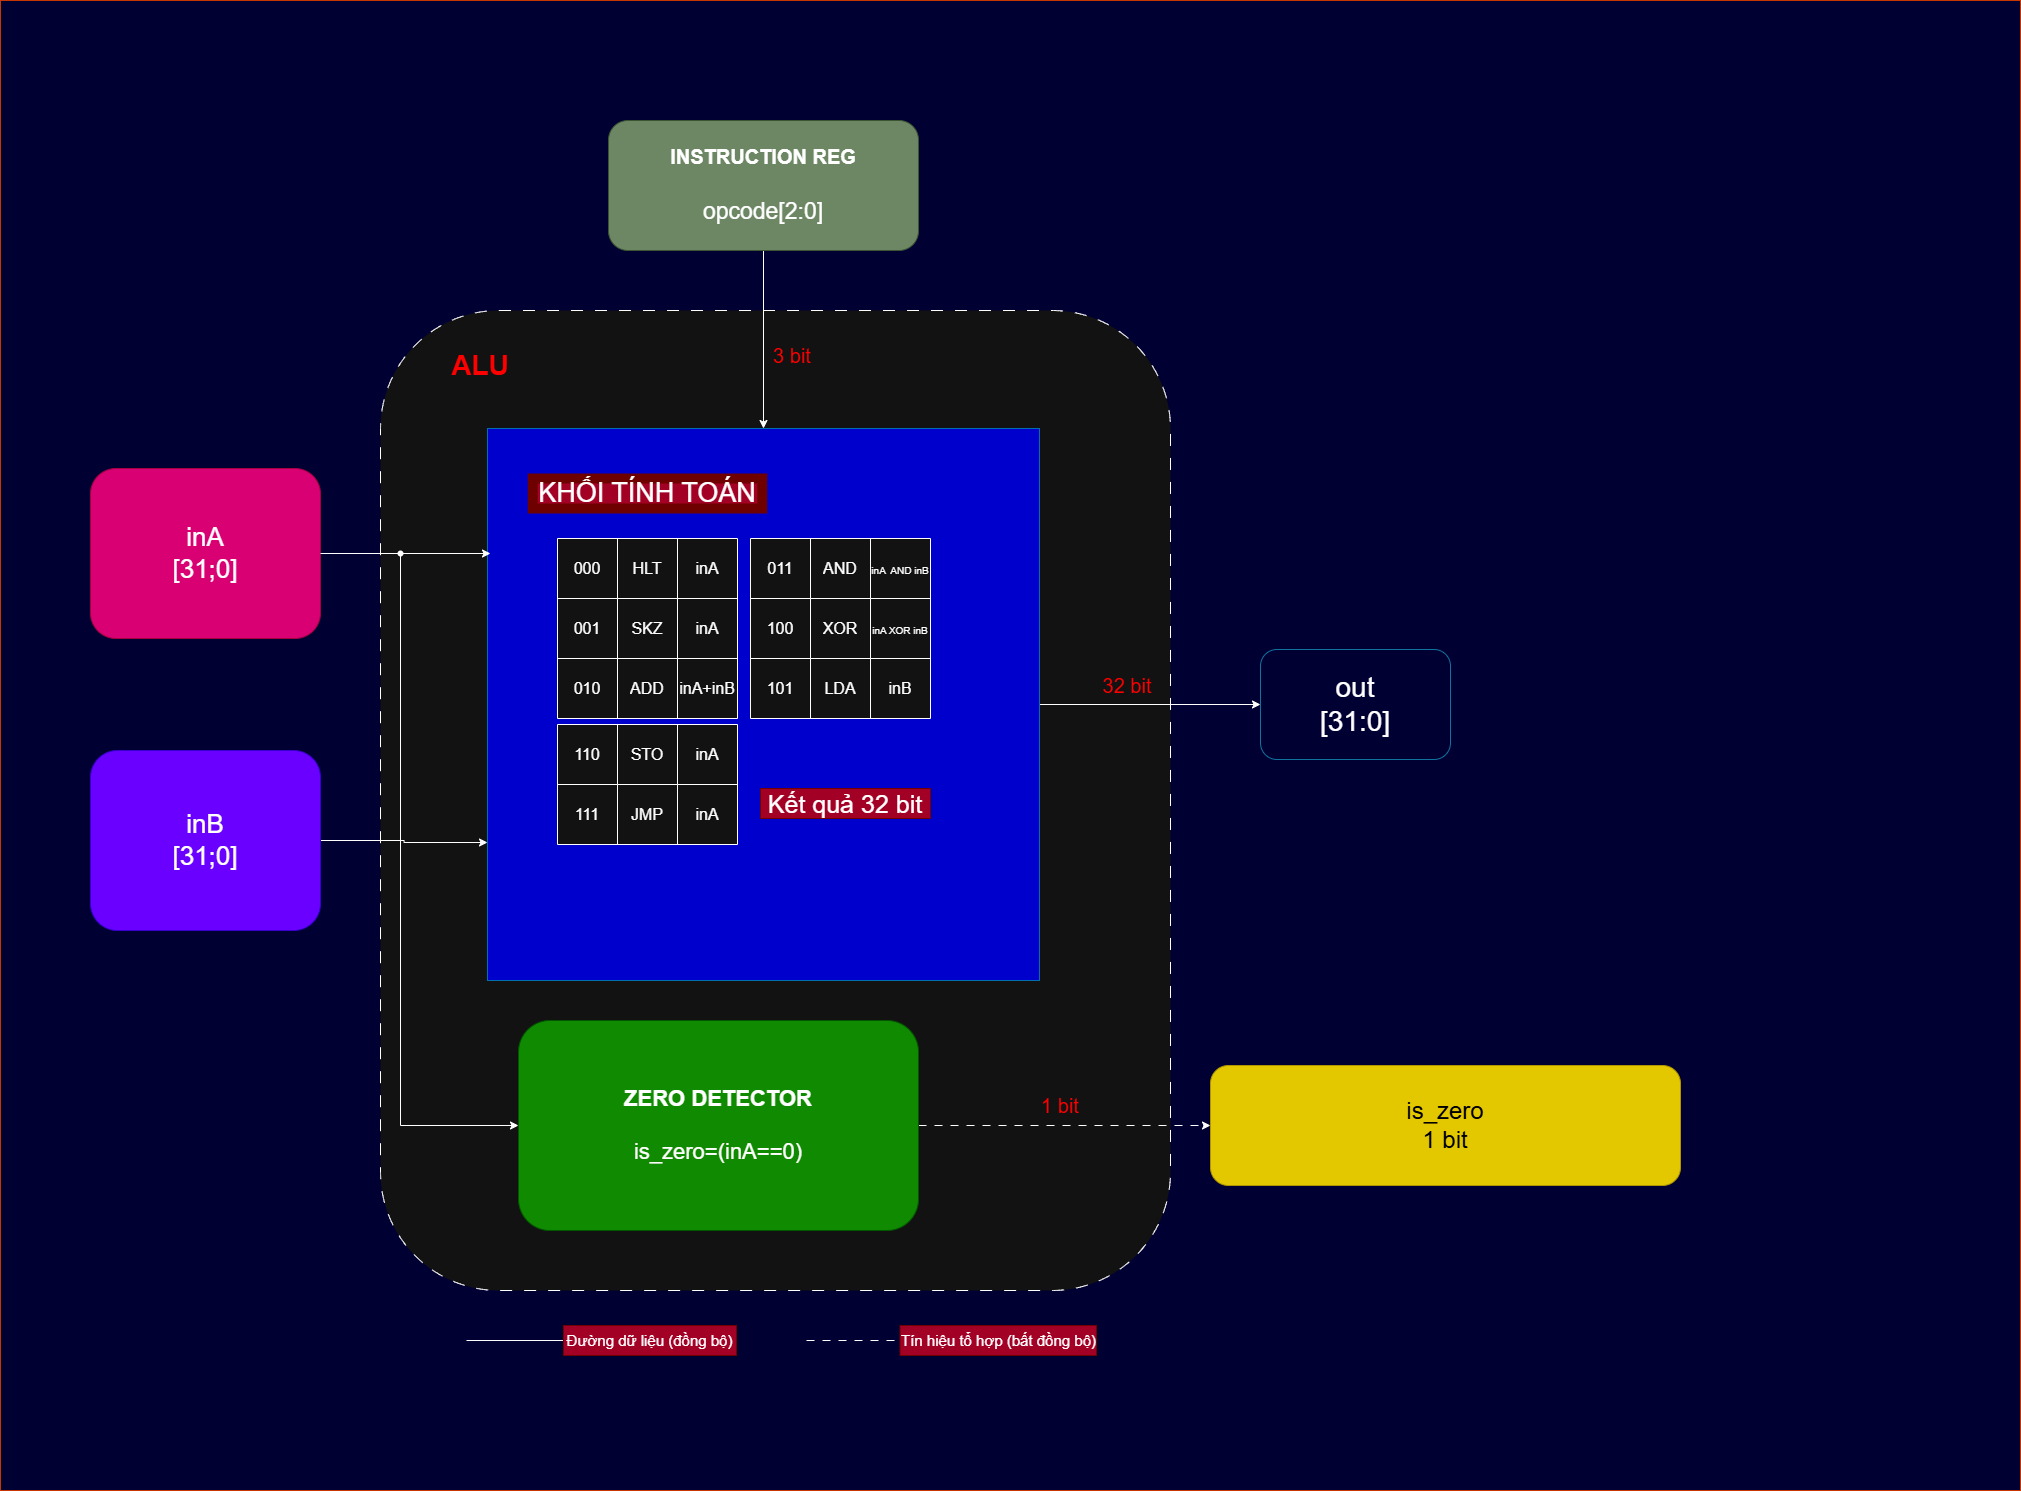
\includegraphics[width=0.9\textwidth]{ALU.png} 
    \caption{Sơ đồ khối tổng quát đơn vị ALU xử lý dữ liệu 32-bit}
    \label{fig:alu_32bit}
\end{figure}

\textbf{Nguyên lý thực thi các phép toán chi tiết:}
Dựa trên Opcode 3-bit từ khối điều khiển, ALU sẽ kích hoạt các mạch logic tương ứng để xử lý hai toán hạng 32-bit ($inA$ và $inB$):

\begin{itemize}
    \item \textbf{Phép cộng (ADD - Opcode 010):} 
    Thực hiện cộng đại số hai giá trị 32-bit. Kết quả $ALU\_Out = inA + inB$. Phép toán này sử dụng bộ cộng đầy đủ (Full Adder) 32-bit để xử lý dữ liệu từ Accumulator và bộ nhớ.
    
    \begin{figure}[H]
        \centering
        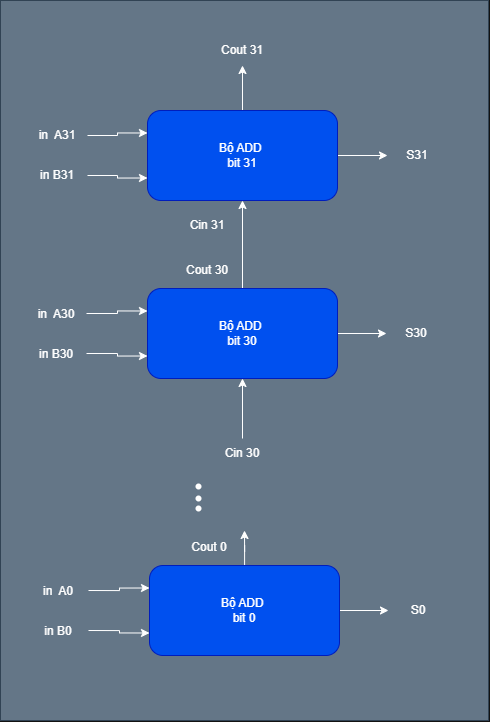
\includegraphics[width=0.8\textwidth]{add.png} % Thay tên file sơ đồ phép ADD vào đây
        \caption{Sơ đồ khối logic cho phép toán ADD 32-bit}
    \end{figure}

    \item \textbf{Phép logic AND (Opcode 011):} 
    Thực hiện phép toán bitwise AND giữa $inA$ và $inB$ trên toàn bộ 32 bit. Kết quả đầu ra chỉ bằng 1 tại các vị trí bit mà cả hai đầu vào đều bằng 1.
    
    \begin{figure}[H]
        \centering
        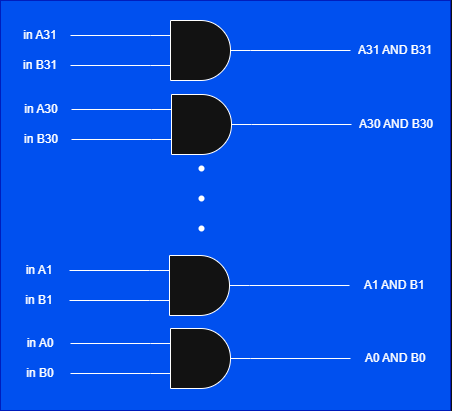
\includegraphics[width=0.9\textwidth]{and.png} % Thay tên file sơ đồ phép AND vào đây
        \caption{Sơ đồ khối logic cho phép toán AND 32-bit}
    \end{figure}

    \item \textbf{Phép logic XOR (Opcode 100):} 
    Thực hiện phép toán bitwise XOR giữa hai toán hạng 32-bit. Phép toán này đặc biệt hữu ích trong việc kiểm tra sự khác biệt hoặc đảo bit dữ liệu.
    
    \begin{figure}[H]
        \centering
        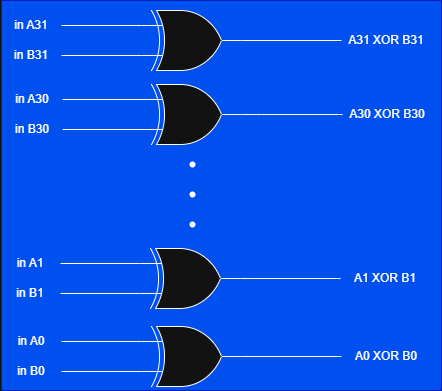
\includegraphics[width=0.6\textwidth]{xor.png} % Thay tên file sơ đồ phép XOR vào đây
        \caption{Sơ đồ khối logic cho phép toán XOR 32-bit}
    \end{figure}
\end{itemize}

\textbf{Tín hiệu Zero Flag ($is\_zero$):}
Một đầu ra quan trọng khác của ALU là tín hiệu $is\_zero$ được tính toán bất đồng bộ. Nếu toàn bộ 32 bit của kết quả đầu ra đều bằng 0, tín hiệu này sẽ được kéo lên mức logic 1. Đây là cơ sở để thực hiện lệnh nhảy có điều kiện \textbf{SKZ} (Skip if Zero).